\section{Experiments}
\label{sec:experiments}

In this section, we conduct the following qualitative and quantitative studies: 1) We visualize the embedding space and show that GN-GloVe separates the protected gender attribute from other latent aspects; 2) We measure the ability of GN-GloVe to distinguish between gender-definition words and gender-stereotype words on a newly annotated dataset;  3) We evaluate GN-GloVe on standard word embedding benchmark datasets and show that it performs well in estimating word proximity; 4) We demonstrate that GN-Glove reduces gender bias on a downstream application, coreference resolution.

We compare GN-GloVe with two embedding models, GloVe and Hard-GloVe. GloVe is a widely-used model~\cite{glove}, and we apply the post-processing step introduced in~\cite{kaiwei} to reduce gender bias in GloVe and name it after Hard-GloVe.
%Hard-GloVe removes gender information in a post-processing manner with the hard debiasing approach.
%Qualitative analysis shows that De-GloVe can successfully constrain the gender information in the gender dimensions while  quantitative analysis on several benchmark datasets demonstrate that  
%  In all the experiments,  We also present qualitative analysis to demonstrate that 
%De-GloVe can successfully isolate the protected variable while preserving word proximity. In the end, 
% In the end, we test the embeddings by coreference resolution which is a downstream application. 
%The experimental results show that the embeddings trained with L1 and L2 are similar. 
All the  embeddings are trained on \textit{2017 English Wikipedia dump} with the default hyper-parameters decribed in ~\cite{glove}.
% After tokenizing and lower-casing the corpus, we build a vocabulary of 322,636 most frequent words.
When training GN-GloVe, we constrain the value of each dimension within $[-1, 1]$ to avoid numerical difficulty.
We set $\lambda_d$ and $\lambda_e$ both to be 0.8. In our preliminary study on development data, we observe that the model is not sensitive to these parameters. 
%Experiments with more hyper-parameter settings are presented in Table~\ref{tab:sims2}. 
%As the main object of this work is to provide a new way to train the word embeddings, we do not fine tune the hyperparamters to get a best performance in some specific tasks. However many 
Unless other stated, we use $J_D^{L1}$ in the GN-GloVe model.
% and for L2-loss, $\lambda_d = 0.6$, $\lambda_e = 0.6$. In practice, assigning  $\lambda_d$ and $\lambda_e$ with a large value encourage the model to move the gender information into the protected dimension $w^{(g)}$.  
% \kw{How you tune the parameters and find these two numbers? This looks like the selection of the parameter is arbitrary and the model is sensitive to the parameter setting so you pick different parameters for L1 and l2. Also, could you put the minus sign for the L2 objective to make the parameter a positive value? It looks weird that we have to set a negative value.} 


\begin{figure*}[!t]
    \begin{subfigure}[b]{0.32\textwidth}
        \hspace{-0.7em}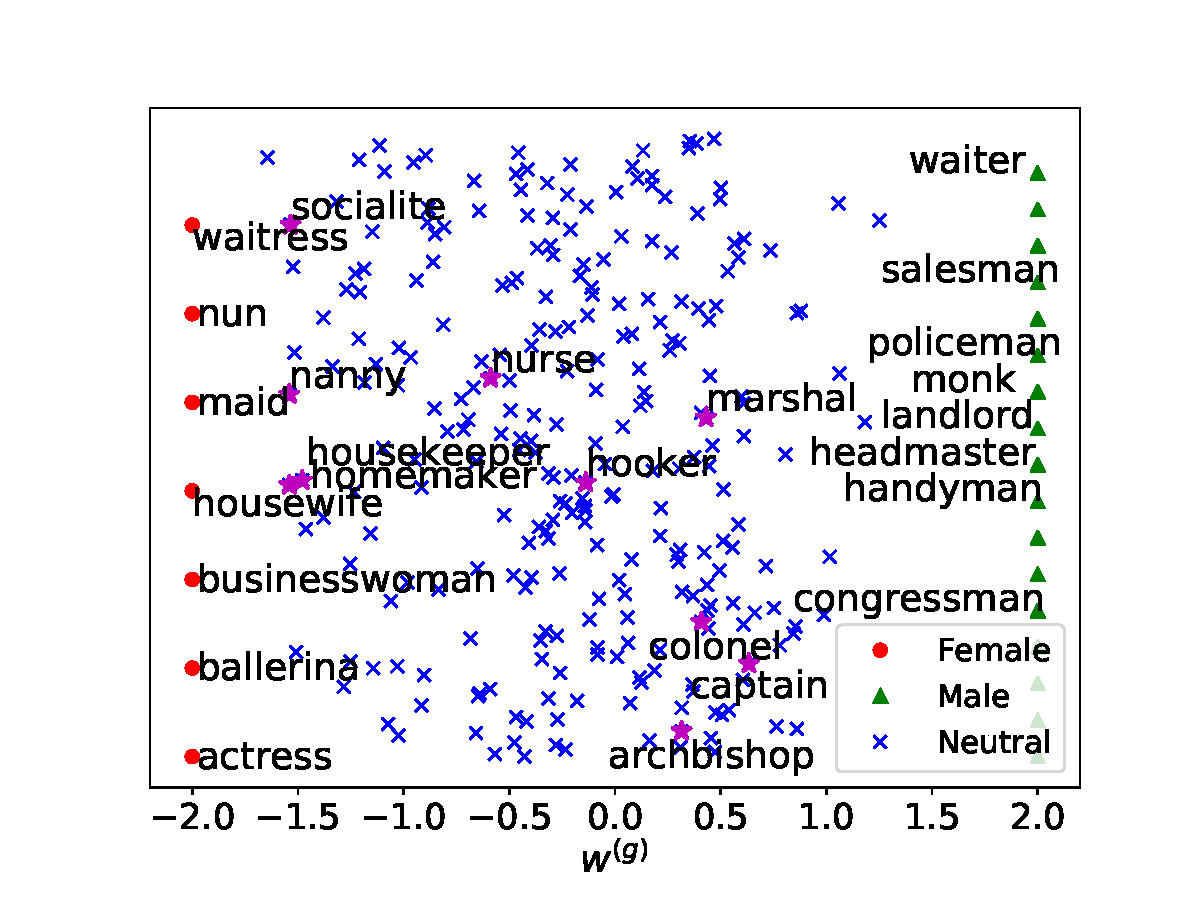
\includegraphics[width=1.14\textwidth]{wg.pdf}
        \caption{
        $w^{(g)}$ dimension for all the professions
        }
        \label{fig:Wg}
    \end{subfigure}
    ~
    \begin{subfigure}[b]{0.32\textwidth}
        \hspace{-1em}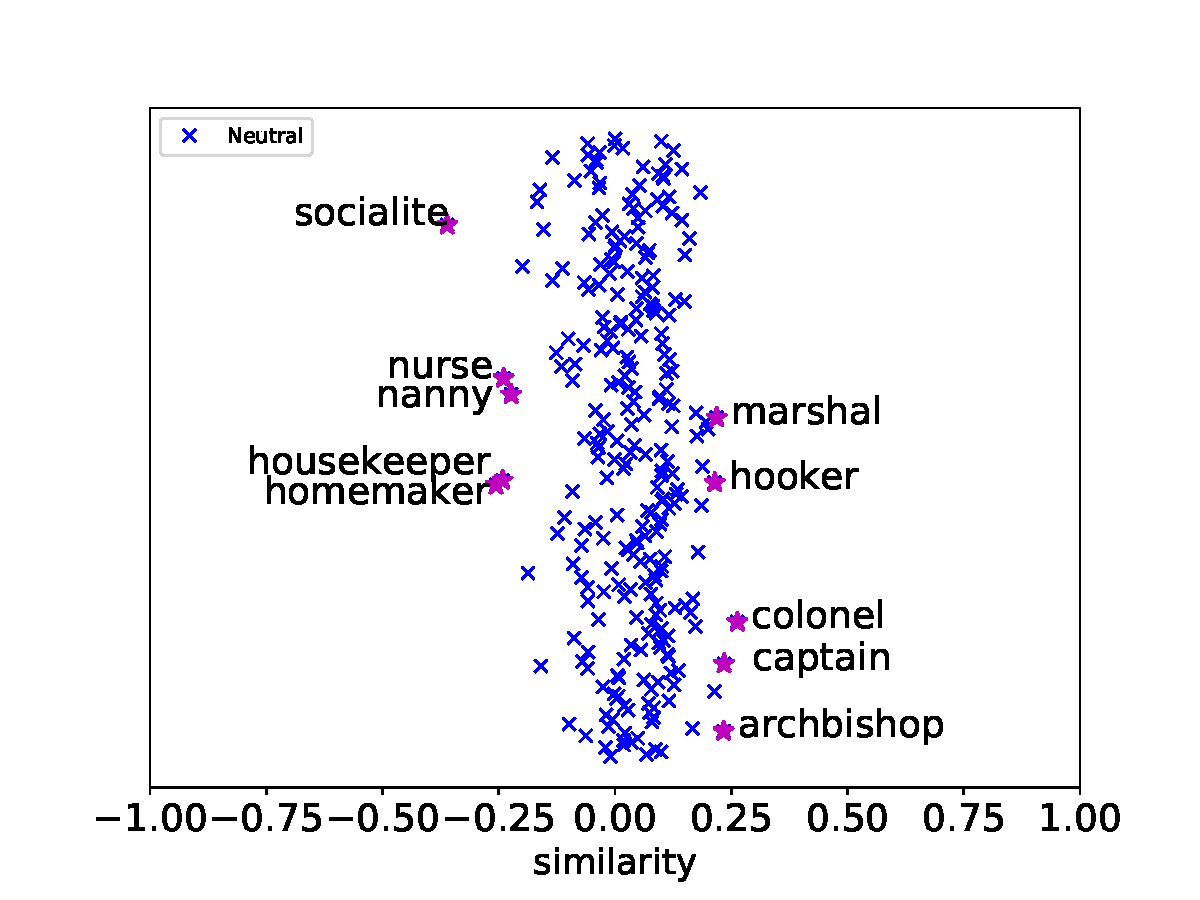
\includegraphics[width=1.14\textwidth]{wa_glove.pdf}
        \caption{
        Gender-neutral profession words projected to gender direction in GloVe
        }
        \label{fig:GloVe}
    \end{subfigure}
    ~ 
    \begin{subfigure}[b]{0.32\textwidth}
        \hspace{-0.8em}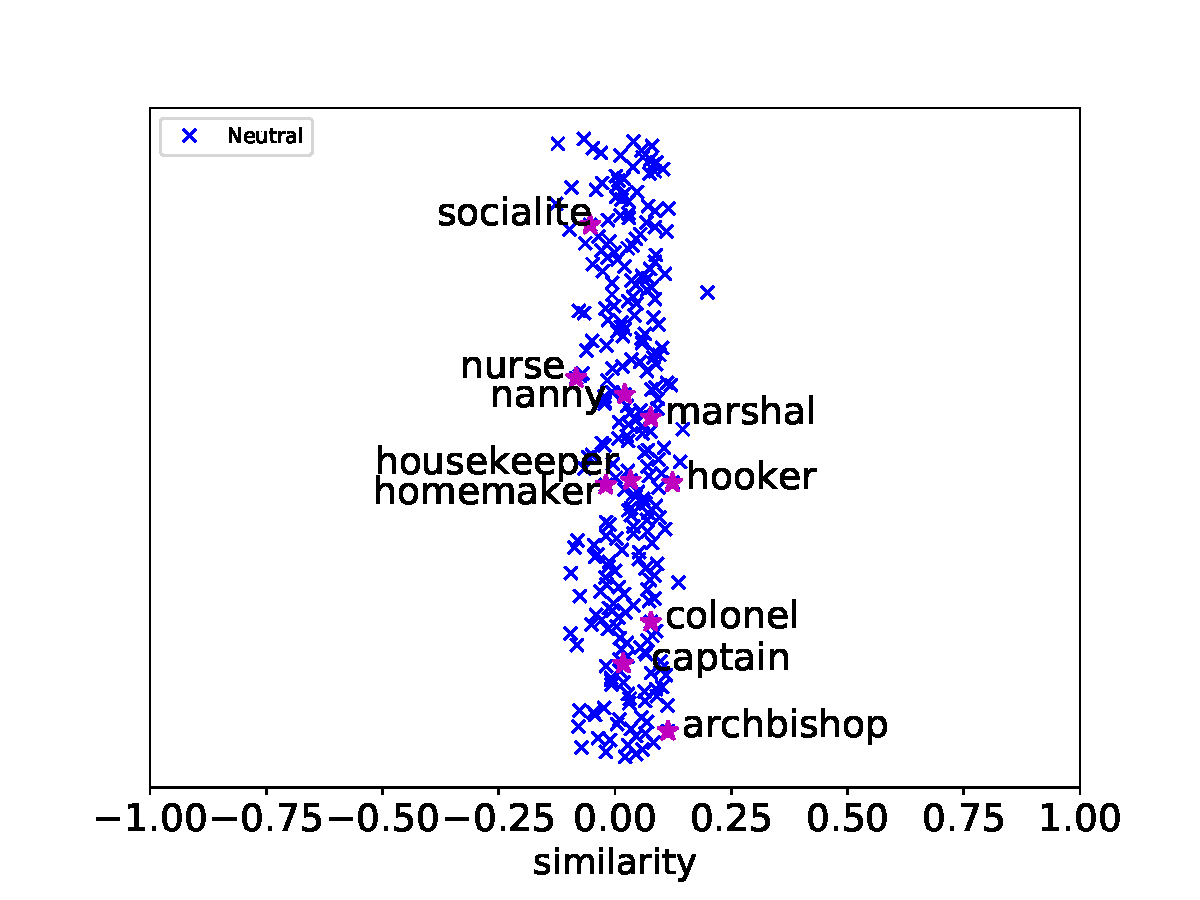
\includegraphics[width=1.14\textwidth]{wa.pdf}
        \caption{
        Gender-neutral profession words projected to gender direction in  GN-GloVe
        }
        \label{fig:De-GloVe}
    \end{subfigure}
    \caption{
    Cosine similarity between the gender direction and the embeddings of gender-neutral words. %The stars are used to highlight several samples.
    In each figure, negative values represent a bias towards female, otherwise male.
    %The comparison between Fig.~\ref{fig:GloVe} and Fig.~\ref{fig:De-GloVe} proves that De-GloVe can remove the gender information from gender-neutral words while $w^{(g)}$ in Fig.~\ref{fig:Wg} preserves the gender information.
    % For example, ``housekeeper" is moved closer to 0 in Fig.~\ref{fig:De-GloVe} than in ~\ref{fig:GloVe} while showing an inclination to female direction  in Fig.~\ref{fig:Wg}, which proves that De-GloVe can successfully separate gender and other information. 
    }
    % \vspace{-8pt}
    \label{fig:comparison}
\end{figure*}

\paragraph{Separate protected attribute} 
First, we demonstrate that GN-GloVe preserves the gender association (either definitional or stereotypical associations) in $w^{(g)}$\footnote{We follow the original GloVe implementation using the summation of word vector and context vector to represent a word. Therefore, the elements of the word vectors are constrained in [-2, 2]}.
To illustrate the distribution of gender information of different words, we plot 
Fig.~\ref{fig:Wg} using $w^{(g)}$ for the x-axis and a random value for the y-axis to spread out words in the plot. As shown in the figure, the gender-definition words, e.g. ``waiter'' and ``waitress'', fall far away from each other in $w^{(g)}$. In addition, words such as ``housekeeper'' and ``doctor'' are inclined to different genders and their $w^{(g)}$ preserves such information. 

Next, we demonstrate that GN-GloVe reduces gender stereotype using a list of profession titles from~\cite{kaiwei}. All these profession titles are neutral to gender by definition.
In Fig.~\ref{fig:GloVe} and Fig.~\ref{fig:De-GloVe},
we plot the cosine similarity between each word vector $w^{(a)}$ and the gender direction ${v_g}$ (i.e.,  $\frac{w^T v_g}{\norm{w}\norm{v_g}}$). Result shows that words, such as ``doctor'' and ``nurse'', possess no gender association by definition, but their GloVe word vectors exhibit strong gender stereotype. In contrast, the gender projects of GN-GloVe word vectors $w^{(a)}$ are closer to zero. This demonstrates the gender information has been substantially diminished from $w^{(a)}$ in the GN-GloVe embedding.

%We split the list into male, female and gender-neutral subsets. As shown in the results (Fig.~\ref{fig:GloVe} and Fig.~\ref{fig:De-GloVe}), their $w^{(a)}$'s are free of gender information as we expect. The projections(cosine similarity) to the gender direction are also much closer to zero, compared with GloVe.

% \paragraph{Occupational stereotypes} 
We further quantify the gender information exhibited in the embedding models.
For each  model, we project the word vectors of occupational words into the gender sub-space defined by ``he-she'' and compute their average size.   A larger projection indicates an embedding model is more biased. Results show that the average projection of GloVe is 0.080, the projection of Hard-GloVe is 0.019, and the projection of Gn-Glove is 0.052. Comparing with GloVe, GN-GloVe reduces the bias by $35\%$. 
Although Hard-GloVe contains less gender information, we will show later GN-GloVe can tell difference between gender-stereotype and gender-definition words better.

\paragraph{Gender Relational Analogy} 
To study the quality of the gender information present in each model, we follow SemEval 2012 Task2~\cite{jurgens2012semeval} to create an analogy dataset, \textit{SemBias}, with the goal to identify the correct analogy of ``he - she'' from four pairs of words. Each instance in the dataset consists of four word pairs: a gender-definition word pair (Definition; e.g., ``waiter - waitress''), a gender-stereotype word pair (Stereotyp; e.g., ``doctor - nurse'') and two other pairs of words that have similar meanings (None; e.g.,  ``dog - cat'', ``cup - lid'')\footnote{The pair is sampled from the list of word pairs with ``SIMILAR: Coordinates'' relation annotated in ~\cite{jurgens2012semeval}. The original list has 38 pairs. After removing gender-definition word pairs, 29 are left.}. We consider 20 gender-stereotype word pairs and 22 gender-definition word pairs and use their Cartesian product to generate 440 instances. Among the 22 gender-definition word pairs, there are 2 word pairs that are not used as a seed word during the training. To test the generalization ability of the model, we generate a subset of data  (SemBias (subset)) of 40 instances associated with these 2 pairs.


% To test if an embedding  can tell the difference between definitions gender association and stereotypical gender association,inspired by SemEval 2012 Task2~\cite{jurgens2012semeval}, we collect 20 gender-definition (e.g., ``waiter - waitress'') and 20 gender-stereotype (e.g., ``doctor - nurse'') word pairs. We create an analogy dataset, {\it SemBias}, consisting 400 instances. Each instance contains 4 word pairs: one definition pair, one stereotype pair, and two pairs of words that have similar meanings (e.g., ``dog - cat'', ``cup - lid'').\footnote{The word pair is sampled from the list of  word pairs with ``SIMILAR: Coordinates'' relation annotated in ~\cite{jurgens2012semeval}. The original list has 38 pairs. After removing word pairs with gender-definition relations, 29 are left.}
%For each instance, we rank the four word pairs by their similarities to ``he-she''% based on the embedding models
%~\cite{mikolov2013linguistic}. We evaluate different embeddings on the whole SemBias dataset as well as SemBias dataset. SemBias  is a subset of  SemBias  where the gender-definition word does not occur as the seed word during training.   Evaluating on SemBias provides us an insight about how well the embeddings can tell the difference between different  categories. By evaluating on , we can show the generalization ability of the embeddings to distinguish gender definitional words with gender stereotypical words.
% reports the percentage of times each class of pair is selected. 
%The goal is to evaluate the proximity of these four pairs to  the ``he: she''.  
% We calculate their cosine similarities with ``he-she'' and choose the largest as the prediction. 
%It is considered a correct prediction when the highest similarity falls on the gender-definition pair.
Table~\ref{tab:isSim} lists the percentage of times that each class of pair is on the top based on a word embedding model~\cite{mikolov2013linguistic}. GN-GloVe achieves 97.7\% accuracy in identifying gender-definition word pairs as an analogy to ``he - she''. In contrast, GloVe and Hard-GloVe makes significantly more mistakes. On the subset, GN-GloVe also achieves significantly better performance than Hard-Glove and GloVe, indicating that it can generalize the gender pairs on the training set to identify other gender-definition word pairs. 

%. On, GN-GloVe achieves 75\% accuracy while Hard-GloVe only gets 25\% indicating GN-GloVe has a better  generalization.
%Mistakes of Hard-GloVe are caused by the errors propagated from incorrect predictions of the gender word classifier, as mentioned in Section~\ref{tab:intro}. 

% To further verify the performance on unseen gender definition words, we exclude all the seed words used for training and do the same experiment on a new  dataset with 40 test instances. GN-GloVe achieves 75\% accuracy while Hard-GloVe only gets 25\% indicating GN-GloVe has a better distinguishing ability. 
 
%Error analysis shows that the mistakes made by Hard-GloVe come from the incorrect predictions of the gender word classifier. 
%makes correction predictions   while  GloVe and Hard-GloVe fail on over 10\% test instances.
% For the hard debiased version, 
%\jy{We analyze the wrong predictions by Hard-GloVe and find it is because of the seed words chosen which also indicates the drawback of this method.}
% Hard-GloVe violently removes the gender information, %from the word embedding, which could 
% which will cause some confusion when evaluating on the properties related to human. 
% Specifically, we find that Hard-GloVe predicts ``pen: pencil'' to be closer to ``he: she'' than ``policeman: policeman'', whereas De-GloVe and De-GloVe-$w_a$ both make correct predictions as ``policeman: policeman''.  


%achieves a better neutralizing performance, it thoroughly eliminates the gender attribute, contradicting our intention of preserving the useful gender information.
% \begin{table}
% \centering
% \resizebox{\linewidth}{!}{
% \begin{tabular}{lcc|cc}
% \hline
% \multirow{2}{*}{Model} & \multicolumn{2}{c|}{Analogy} & \multicolumn{2}{c}{Similarity} \\
% \cline{2-5}
%      & Google & MSR  & WS353-ALL & MTurk-771\\
% \hline
% GloVe      & \textbf{70.8} & \textbf{45.8} & 62.0          & 64.9\\
% Hard-GloVe & \textbf{70.8} & \textbf{45.8} & 61.2          & 64.8\\
% GN-GloVe-L1& 68.9          & 43.7          & \textbf{62.8} &  
% \textbf{66.2}\\
% GN-GloVe-L2& 68.8          & 43.6          & 62.5          & 65.6\\
% \hline
% \end{tabular}
% }
% \caption{Performance on the word embeddings evaluation tasks, given as percent accuracy.  %We retrain GloVe using the same parameters as De-GloVe. Hard-GloVe is generated by applying the hard debiasing method to GloVe.
% }
% % \vspace{-9pt}
% \label{tab:sims}
% \end{table}

\begin{table}
\centering
\resizebox{\linewidth}{!}{
\begin{tabular}{ll|ccc}
\hline
Dataset & Embeddings & Definition & Stereotype & None\\
\hline
\multirow{ 3}{*}{SemBias} & GloVe      & 80.2       & 10.9       & 8.9 \\
% De-GloVe-$w_a$        & 300        & 0  \\
& Hard-Glove &  84.1       &   6.4       &  9.5 \\
& GN-GloVe   &   97.7      &    1.4        &  0.9  \\
\hline
\multirow{ 3}{*}{\shortstack[l]{SemBias\\(subset)}} & GloVe      &  57.5       &   20      & 22.5 \\
% De-GloVe-$w_a$        & 300        & 0  \\
& Hard-Glove &    25     &  27.5       & 47.5 \\
& GN-GloVe   & 75        & 15          & 10  \\
\hline
\end{tabular}
}
\caption{Percentage of predictions for each category on gender relational analogy task. %GD stands for gender-definition pairs, ST refers to the stereotyped pairs and NO means the noise pairs. 
% De-GloVe can make correct predictions on this task while  GloVe and Hard-debiased glove fail on over 10\% test instances.
}
\label{tab:isSim}
\end{table}



\begin{table*}[!thbp]
\centering
\resizebox{\linewidth}{!}{
\begin{tabular}{l|cc|cccccc}
\hline
\multirow{2}{*}{Embeddings} & \multicolumn{2}{c|}{Analogy} & \multicolumn{6}{c}{Similarity} \\
  & Google & MSR & WS353-ALL  & RG-65  & MTurk-287 & MTurk-771 & RW & MEN-TR-3k \\
\hline
GloVe      &    \textbf{70.8} & \textbf{45.8 }    & 62.0    & 75.3   & 64.8    & 64.9   & 37.3    & 72.2 \\
Hard-GloVe &   \textbf{70.8} & \textbf{45.8}     & 61.2    & 74.8   & 64.4    & 64.8   & 37.3    & 72.2 \\
GN-GloVe-L1&   68.9 & 43.7   & \textbf{62.8}   & 74.1   & 66.2    & \textbf{66.2}   & \textbf{40.0}    & \textbf{74.5} \\
GN-GloVe-L2&   68.8 & 43.6   & 62.5  & \textbf{76.4}   & \textbf{66.8}    & 65.6   & 39.3    & 74.4 \\
%GN-GloVe-L2& (0.6,0.6)  & \textbf{63.2}    & \textbf{76.6}   & 65.5    & 65.8   & 39.7    & \textbf{74.8} \\
%GN-GloVe-L1& (0.3,0.5)  & 62.1    & 74.3   & 64.8    & \textbf{66.6}   & 39.9    & 74.4 \\
%GN-GloVe-L2& (0.3,0.5)  & 62.8    & 75.8   & 66.2    & 66.2   & 39.5    & 74.6 \\
%De-GloVe-L1& (0.5,0.3)  &     &    &     &    &     &  \\
%GN-GloVe-L2& (0.5,0.3)  & 63.0    & 75.3   & 65.1    & 66.2   & 39.8    & 74.4 \\

\hline
\end{tabular}
}
\caption{Results on the benchmark datasets. Performance is measured in accuracy
and in Spearman rank correlation for word analogy and word similarity tasks, respectively.}
% \vspace{-10pt}
\label{tab:sims2}
\end{table*}

\paragraph{Word Similarity and Analogy} In addition, we evaluate the word embeddings on the benchmark tasks to ensure their quality. 
The word similarity tasks measure how well a word embedding model captures the similarity between words comparing to human annotated rating scores. Embeddings are tested on multiple datasets:  WS353-ALL~\cite{finkelstein2001placing}, RG-65~\cite{rubenstein1965contextual},  MTurk-287~\cite{radinsky2011word}, MTurk-771~\cite{halawi2012large}, RW~\cite{luong2013better}, and MEN-TR-3k~\cite{bruni2012distributional} datasets.  
% In word similarity tasks such as WS353~\cite{finkelstein2001placing}, MTurk287~\cite{radinsky2011word}, RW-STANFORD~\cite{luong2013better}, and MEN-TR-3k~\cite{bruni2012distributional},
% word similarity scores computed by word embeddings are compared with corresponding similarity ratings judged by human annotators.
% This task measures how well the word embeddings preserve the word similarities. 
% a list of word pairs along with their similarity ratings judged by human annotators are provided to measure how well the similarity can be captured by the word embeddings~\cite{finkelstein2001placing}.
The analogy tasks are to answer the question ``\textit{A} is to \textit{B} as \textit{C} is to \underline{\hbox to 2mm{}}?'' by finding a word vector $w$ that is closest to $w_A - w_B + w_C$ in the embedding space.
Google~\cite{mikolov2013efficient} and MSR~\cite{mikolov2013linguistic} datasets are utilized for this evaluation. 
% The first dataset consists of 19,544  questions divided into semantic and syntactic parts while the MSR dataset consists 8,000 questions all of which belong to the syntactic category. 
% The semantic questions are about places or people such as ``Beijing is to China as Berlin is to \underline{\hbox to 3mm{}}?'' The syntactic questions are like ``dance is to dancing as teach is to \underline{\hbox to 3mm{}}?''
% To answer such questions, the model needs to identify the missing term and only the exact correspondence will be counted as the correct answer. 
The results are shown in Table ~\ref{tab:sims2}, where the suffix ``-L1'' and ``-L2'' of GN-GloVe stand for the GN-GloVe  using  $J_D^{L1}$ and $J_D^{L2}$, respectively. 
Compared with others, GN-GloVe achieves a higher accuracy in the similarity tasks and its analogy score slightly drops indicating that GN-GloVe is capable of preserving proximity among words. 

\paragraph{Coreference Resolution} Finally, we investigate how the gender bias in word embeddings affects a downstream application, such as coreference resolution.
Coreference resolution aims at clustering the denotative noun phrases referring to the same entity in the given text. We evaluate our models on the Ontonotes 5.0~\cite{weischedel2012ontonotes} benchmark dataset and the WinoBias dataset~\cite{zhao2018gender}.\footnote{Specifically, we conduct experiments on the Type 1 version. } In particular, the WinoBias dataset is composed of pro-stereotype (PRO) and anti-stereotype (ANTI) subsets. 
%As shown in~\cite{zhao2018gender}, word embeddings can cause gender bias issues in such tasks~\cite{zhao2018gender} by linking gender pronoun ``he'' and ``she'' to different stereotyped professions. We evaluate our word embeddings on the WinoBias dataset they proposed\footnote{They have two different types of dataset, here we only evaluate on the Type1 dataset.}.
% such as linking ``doctor'', or ``developer'' to ``he''and  ``teacher'', or ``nurse'' to ``she'' more frequently than the opposite case. 
% for example, it contains the sentence like 
 The PRO subset consists of sentences where a gender pronoun refers to a profession, which is dominated by the same gender.
 Example sentences include ``The CEO raised the salary of the receptionist because he is generous.'' In this sentence, the pronoun ``he'' refers to ``CEO'' and this reference is consistent with societal stereotype. The ANTI subset contains the same set of sentences, but the gender pronoun in each sentence is replaced by the opposite gender. For instance, the gender pronoun ``he'' is replaced by ``she'' in the aforementioned example. Despite the sentence is almost identical, the gender pronoun now refers to a profession that is less represented by the gender.  Details about the dataset are in ~\cite{zhao2018gender}.
% We provide an instance of the dataset in Fig~\ref{fig:winobias}. For more details, please refer to their paper.
% \begin{figure}
%     \centering
%     \includegraphics[width=0.5\textwidth]{figures/coref.pdf}
%     \caption{Example of WinoBias dataset. The solid purple line stands for the pro-stereotype linking while the dashed line refers to the anti-stereotype linking.}
%     \label{fig:winobias}
% \end{figure}

% We evaluate De-GloVe in the coreference task and  the results are shown in Table~\ref{tab:coref}. 
We train the end-to-end coreference resolution model~\cite{lee2017end} with different word embeddings on OntoNote and report their performance in Table \ref{tab:coref}.
For the WinoBias dataset, we also report the average (Avg) and absolute difference (Diff) of F1 scores on two subsets. A smaller Diff value indicates less bias in a system.
% train the end-to-end model proposed in~\cite{lee2017end} with different word embeddings for about 200k iterations. 
Results show that GN-GloVe achieves comparable performance as Glove and Hard-GloVe on the OntoNotes dataset while distinctly reducing the bias on the WinoBias dataset. 
When only the $w^{(a)}$ potion of the embedding is used in representing words, GN-GloVe($w^{(a)}$) further reduces the bias in coreference resolution. 

%Moreover, if we remove the gender information (i.e., GN-GloVe-$w^{(a)}$), the bias is  further reduced.
% Also we can see that if only use the gender neutral word embeddings, we can do better on the anti-stereotype dataset. 

\begin{table}
\centering
\resizebox{\linewidth}{!}{
\begin{tabular}{l|c|cccc} \hline
Embeddings     &  OntoNotes-test & PRO & ANTI & Avg & Diff\\ 
\hline
GloVe          & 66.5       &  76.2 & 46.0 & 61.1 & 30.2\\
Hard-Glove     & 66.2       & 70.6 & 54.9 & 62.8 & 15.7\\
GN-GloVe       & 66.2       & 72.4 & 51.9  & 62.2 & 20.5 \\
GN-GloVe($w_a$) & 65.9       & 70.0 & 53.9 & 62.0 & 16.1\\
\hline
\end{tabular}
}
\caption{F1 score (\%) on the coreference system. %GN-GloVe-$w_a$ represents words by the $w_a$ portion in GN-GloVe.
}
\vspace{-10pt}
\label{tab:coref}
\end{table}


% \begin{figure*}[!t]
%     \centering
%     \begin{subfigure}[b]{0.31\textwidth}
%         \includegraphics[width=\textwidth]{figures/wa_hard.pdf}
%         \caption{Stereotype in Hard-GloVe}
%         \label{fig:hard}
%     \end{subfigure}
%     ~
%     \begin{subfigure}[b]{0.31\textwidth}
%         
\includegraphics[width=\textwidth]{figures/wa_glove.pdf}
%         \caption{Stereotype   in GloVe}
%         \label{fig:wa_glove}
%     \end{subfigure}
%     ~ %add desired spacing between images, e. g. ~, \quad, \qquad, \hfill etc. 
%     %(or a blank line to force the subfigure onto a new line)
%     \begin{subfigure}[b]{0.31\textwidth}
%         
\includegraphics[width=\textwidth]{figures/wa.pdf}
%         \caption{Stereotype  in De-GloVe}
%         \label{fig:wa_debias}
%     \end{subfigure}
%     \caption{Stereotyped professions mapped to gender direction in Hard-GloVe, GloVe and De-GloVe. For all these figures, x-axis is the $w^{(g)}$ dimension which is learned from De-GloVe. For GloVe and Hard-GloVe, this x-axis is used to align the professions among images. Y-axis is the projection to the gender direction using $w^a$ part (300 dimensions for GloVe and Hard-GloVe; 299 dimensions for De-Glove). The green triangles and red dots represent the stereotyped male and female professions respectively.}
%     \label{fig:occp}
% \end{figure*}

